\documentclass[11pt,a4paper]{article}

% ==================== PACKAGES ====================
\usepackage[T1]{fontenc}
\usepackage[utf8]{inputenc}
\usepackage{lmodern}
\usepackage[margin=2.5cm]{geometry}
\usepackage{amsmath,amssymb}
\usepackage{graphicx}
\usepackage{booktabs}
\usepackage{tabularx}
\usepackage{enumitem}
\usepackage{xcolor}
\usepackage{microtype}
\usepackage[hidelinks]{hyperref}

% ==================== FORMATTING ====================
\setlength{\parindent}{0pt}
\setlength{\parskip}{0.35em}
\setlength{\emergencystretch}{2em}
\setlist[itemize]{nosep,leftmargin=*}
\setlist[enumerate]{nosep,leftmargin=*}

% Set to \draftfalse before submission to hide guidance.
% Hiding guidance does not replace completing the missing content.
\newif\ifdraft
\drafttrue

\newcommand{\todo}[1]{%
  \ifdraft
    \par\noindent
    {\small\color{blue!65!black}\textbf{TO COMPLETE:} #1}
    \par
  \fi
}

\newcommand{\NA}{\textemdash}

% ==================== DOCUMENT ====================
\begin{document}

% ==================== TITLE ====================
\begin{center}
\setlength{\parskip}{0pt}

{\small Mathematical Modelling Project\par}
\vspace{0.2cm}

{\Large\bfseries
Adaptive Debt Collection Routing under Payment Uncertainty\par}

\vspace{0.3cm}

\begin{minipage}[t]{0.48\textwidth}
\centering
\textbf{Nguyen Thang Phuc}\\[2pt]
{\small Student ID: 20252263M}\\[2pt]
\href{mailto:Phuc.NT252263M@sis.hust.edu.vn}
{\scriptsize\texttt{Phuc.NT252263M@sis.hust.edu.vn}}
\end{minipage}
\hfill
\begin{minipage}[t]{0.48\textwidth}
\centering
\textbf{Dinh Thi Lan Huong}\\[2pt]
{\small Student ID: 20261261M}\\[2pt]
\href{mailto:Huong.DTL261261M@sis.hust.edu.vn}
{\scriptsize\texttt{Huong.DTL261261M@sis.hust.edu.vn}}
\end{minipage}

\vspace{0.25cm}

{\small
\textbf{Supervisor:} Viet Hung NGUYEN
\enspace$\vert$\enspace
\href{mailto:viet_hung.nguyen@uca.fr}
{\texttt{viet\_hung.nguyen@uca.fr}}
\par}
\end{center}

% ==================== 1. INTRODUCTION ====================
\section{Introduction}
\label{sec:introduction}

Debt collection requires financial institutions to allocate limited
staff time among customers located in different geographical areas.
When in-person visits are necessary, collection officers must decide
which customers to visit, in what order, and on which days. These
decisions influence both travel requirements and the amount of money
that may be recovered. Visiting every customer is often impractical
because travel and service times must fit within daily working-hour
limits. Furthermore, a visit does not guarantee payment, and an
unsuccessful visit may require a subsequent attempt.

This project considers a multi-officer, multi-day debt collection
routing problem in Hanoi. A team of collection officers operates
from a common branch over a finite planning horizon. Each customer
is associated with a target collection amount, an assumed payment
probability, a service duration, and a geographical location.
Each officer's daily route starts and ends at the branch, and total
travel and service time must remain within the available working
hours. Customers may be revisited subject to a maximum visit
allowance, but a successfully collected amount must not be counted
more than once.

The motivation is to allocate collection effort effectively under
limited operational capacity and uncertain payment outcomes.
Prioritizing nearby customers alone may overlook larger expected
recoveries, whereas prioritizing large debts alone may lead to
excessive travel or repeated unsuccessful visits. The problem
therefore combines customer selection, visit scheduling, and route
construction. The primary objective is to maximize expected
recovered money. A secondary objective is to minimize total travel
distance while preserving the primary objective value within a
specified numerical tolerance.

The planning problem is formulated as a mixed-integer linear
programming model and implemented in Julia using JuMP and the
HiGHS solver. Heuristic approaches, including a genetic algorithm,
tabu search, and adaptive large neighborhood search, are also
investigated. The experimental study is designed to compare
solution quality, computational time, and optimality gaps when
valid solver bounds are available.

Two planning policies are considered. A static policy constructs
a plan for the entire horizon before execution. A rolling-horizon
policy updates customer states after each day and reoptimizes the
remaining plan. Customers who have paid are removed from future
visits, while unsuccessful visits reduce their remaining visit
allowances. Simulated payment outcomes provide a common basis
for comparing these policies.

The study uses a synthetic dataset informed by public demographic
and credit-related data, together with geographical and road-network
information. Customer accounts and payment outcomes are simulated
and do not represent an actual bank's collection records.
Payment probabilities are modelling assumptions rather than
estimates validated against historical collection outcomes.
The project therefore evaluates the behaviour and trade-offs of
the proposed methods under controlled scenarios, rather than
claiming verified improvements in real banking operations.

% ==================== 2. MATHEMATICAL MODEL ====================
\section{Mathematical Model}
\label{sec:model}

\subsection{Problem Assumptions}
A successful visit to customer $i$ collects the full target amount $w_i$ and
an unsuccessful one collects nothing. $p_{it}$ is the probability that
customer $i$ pays when visited on day $t$, given no earlier payment; outcomes
of different visits are conditionally independent and $p_{it}$ decreases
with $t$. Customer $i$ is visited at most $m_i$ times over the horizon
($m_i=2$ in all experiments) and at most once per day, by one officer;
different visits may be made by different officers. All officers can visit
all customers and have equal daily budgets. Every active officer leaves the
branch once per day and returns before the budget, which covers travel and
service time, is used up. A customer who has paid receives no further
visits: in the planning model this is captured by the expected value of a
visit schedule, and during execution by skipping the customer
(Section~\ref{sec:rolling}).

\subsection{Input Data and Notation}
Table~\ref{tab:notation} lists the notation. Money is expressed in
million VND, time in hours and distance in kilometers. Travel times and
distances come from shortest (fastest) paths on a directed motorbike road
network, so in general $d_{ij}\ne d_{ji}$ and $\tau_{ij}\ne\tau_{ji}$.

\begin{table}[htbp]
\centering
\caption{Main notation.}
\label{tab:notation}
\small
\begin{tabularx}{\linewidth}{@{}lX@{}}
\toprule
Symbol & Description \\
\midrule
$N$ & Set of customers \\
$K$ & Set of collection officers \\
$T$ & Set of planning days \\
$V=N\cup\{0\}$ & Routing nodes, where $0$ is the branch \\
$A=\{(i,j)\in V\times V: i\ne j\}$ & Arcs of the complete directed routing graph \\
$n=|N|$ & Number of customers \\
$w_i$ & Target collection amount of customer $i$ (million VND) \\
$p_{it}$ & Payment probability for customer $i$ on day $t$, given no earlier payment \\
$d_{ij}$ & Travel distance from node $i$ to node $j$ (km) \\
$\tau_{ij}$ & Travel time from node $i$ to node $j$ (hours) \\
$s_i$ & Service duration at customer $i$ (hours) \\
$B_{kt}$ & Working-time budget of officer $k$ on day $t$ (hours; 8 h in all instances) \\
$m_i$ & Maximum number of visits to customer $i$ \\
$\mathcal S_i$ & Feasible visit schedules of customer $i$: $\{S\subseteq T: 1\le|S|\le m_i\}$ \\
$a_{tS}$ & $1$ if $t\in S$, $0$ otherwise \\
$v_{iS}$ & Precomputed expected collection of customer $i$ under schedule $S$ (million VND) \\
\bottomrule
\end{tabularx}
\end{table}

\subsection{Decision Variables}
All variables are indexed by $i,j\in V$, $k\in K$, $t\in T$ and
$S\in\mathcal S_i$.
\begin{itemize}
\item $x_{ijkt}\in\{0,1\}$, $(i,j)\in A$: equals 1 if officer $k$ travels
  directly from node $i$ to node $j$ on day $t$ (arc variables).
\item $y_{ikt}\in\{0,1\}$, $i\in N$: equals 1 if officer $k$ visits customer
  $i$ on day $t$ (visit assignment).
\item $z_{kt}\in\{0,1\}$: equals 1 if officer $k$ performs a route on day
  $t$ (route activation).
\item $\lambda_{iS}\in\{0,1\}$, $i\in N$: equals 1 if customer $i$ is
  visited exactly on the set of days $S$ (schedule selection).
\item $u_{ikt}\ge 0$, $i\in N$: position of customer $i$ in the route of
  officer $k$ on day $t$; used only for subtour elimination
  (Miller--Tucker--Zemlin variables~\cite{mtz1960}).
\end{itemize}

\subsection{Objective Function}
With full-or-zero payment and conditionally independent visits, the
probability that customer $i$ pays at least once under schedule $S$ is
$1-\prod_{t\in S}(1-p_{it})$, so its expected collection is
\begin{equation}
v_{iS}=w_i\Bigl[1-\prod_{t\in S}\bigl(1-p_{it}\bigr)\Bigr].
\label{eq:schedule-value}
\end{equation}
This value is not additive over the visits: a second visit only adds value
if the first one fails. Expressing it directly in terms of $y_{ikt}$ would
require products of binary variables. Instead, $v_{iS}$ is computed before
solving for every schedule in $\mathcal S_i$, and the model selects one
schedule per customer. The objective is therefore linear:
\begin{equation}
\max\; Z=\sum_{i\in N}\sum_{S\in\mathcal S_i} v_{iS}\,\lambda_{iS}.
\label{eq:objective}
\end{equation}
With $H=5$ days and $m_i=2$, each customer has
$|\mathcal S_i|=\binom51+\binom52=15$ schedules.

\textbf{Secondary objective.} Let $Z^\star$ be the value obtained in the first
solve. A second solve keeps the expected collection within a relative
tolerance $\varepsilon=10^{-6}$ and minimizes the total distance:
\begin{align}
&\sum_{i\in N}\sum_{S\in\mathcal S_i} v_{iS}\lambda_{iS}
  \;\ge\; Z^\star-\varepsilon\max(1,|Z^\star|), \label{eq:lexi}\\
&\min\;\sum_{t\in T}\sum_{k\in K}\sum_{(i,j)\in A} d_{ij}\,x_{ijkt}.
  \label{eq:distance}
\end{align}
The second solve starts from the first solution and has its own time limit.
In the experiments it is run only when the first solve is proved optimal,
with the same time limit as the first solve. In the heuristics, distance is always used as a lexicographic
tie-breaker between solutions with equal expected value.

\subsection{Constraints}
\begin{align}
&\sum_{S\in\mathcal S_i}\lambda_{iS}\le 1
  && \forall i\in N, \label{eq:c-schedule}\\
&\sum_{k\in K} y_{ikt}=\sum_{S\in\mathcal S_i} a_{tS}\lambda_{iS}
  && \forall i\in N,\ t\in T, \label{eq:c-link}\\
&\sum_{j\in N} x_{0jkt}=z_{kt},\qquad \sum_{i\in N} x_{i0kt}=z_{kt}
  && \forall k\in K,\ t\in T, \label{eq:c-depot}\\
&\sum_{j\in V\setminus\{i\}} x_{ijkt}=y_{ikt},\qquad
 \sum_{j\in V\setminus\{i\}} x_{jikt}=y_{ikt}
  && \forall i\in N,\ k\in K,\ t\in T, \label{eq:c-flow}\\
&\sum_{(i,j)\in A}\tau_{ij}x_{ijkt}+\sum_{i\in N}s_i y_{ikt}\le B_{kt}z_{kt}
  && \forall k\in K,\ t\in T, \label{eq:c-time}\\
&u_{ikt}-u_{jkt}+n\,x_{ijkt}\le n-1+n(1-y_{jkt})
  && \forall i,j\in N,\ i\ne j,\ k\in K,\ t\in T, \label{eq:c-mtz}\\
&y_{ikt}\le u_{ikt}\le n\,y_{ikt}
  && \forall i\in N,\ k\in K,\ t\in T, \label{eq:c-order}\\
&x_{ijkt},\,y_{ikt},\,z_{kt},\,\lambda_{iS}\in\{0,1\},\quad u_{ikt}\ge 0. \label{eq:c-domain}
\end{align}

Constraint~\eqref{eq:c-schedule} gives each customer at most one schedule
(a customer may be skipped; $m_i$ is enforced through $\mathcal S_i$).
Constraint~\eqref{eq:c-link} makes exactly one officer visit customer $i$ on
each day of its schedule and nobody on other days.
Constraints~\eqref{eq:c-depot}--\eqref{eq:c-flow} make an active officer
leave and re-enter the branch once and give every visited customer one
incoming and one outgoing arc on the route of its officer.
Constraint~\eqref{eq:c-time} limits travel plus service time to $B_{kt}$.
In the MTZ constraints~\eqref{eq:c-mtz}--\eqref{eq:c-order}, $x_{ijkt}=1$
with $j$ visited forces $u_{jkt}\ge u_{ikt}+1$, so no cycle can avoid the
branch; the term $n(1-y_{jkt})$ relaxes the constraint when $j$ is not on
the route.

\textbf{Symmetry breaking.} Officers with equal budgets are
interchangeable, so the search tree contains relabelled copies of every
solution. For consecutive officers with $B_{kt}=B_{k+1,t}$ the model adds
\begin{equation}
z_{kt}\ge z_{k+1,t}\qquad k=1,\dots,|K|-1,\ t\in T,
\label{eq:c-symmetry}
\end{equation}
which does not change the optimal value and is used in all experiments.

\subsection{Rolling-Horizon Operation}
\label{sec:rolling}
The model above produces a \emph{static} plan for the whole horizon. During
execution, payment outcomes are revealed day by day. The state known at the
start of day $t$ is $(P_t,a_t)$, where $P_t$ is the set of customers who have
already paid and $a_{it}$ is the number of visits made to customer $i$
before day $t$. The eligible customers are
$A_t=\{i\in N: i\notin P_t,\ a_{it}<m_i\}$.

Each morning $t=1,\dots,H$, the rolling-horizon policy builds the remaining
problem (customers $A_t$, days $t,\dots,H$, remaining visit allowances
$m_i-a_{it}$), solves model~\eqref{eq:objective}--\eqref{eq:c-domain} on it,
executes only the routes of day $t$ and records the simulated payments. The
probabilities are not re-estimated: $p_{it}$ is already conditional on no
earlier payment, so it stays valid for every customer in $A_t$. Two
reference policies are compared with it. The \emph{static} policy executes
the initial plan and skips customers who have already paid, without
inserting new ones. The \emph{myopic} policy re-plans each morning but
optimizes day $t$ only ($H=1$). All three policies produce feasible routes.
The rolling horizon is not a fully adaptive stochastic model: each re-solve
assumes that the remaining plan will be executed without further
re-planning, so it is not an optimal policy of the multi-stage problem.

% ==================== 3. SOLUTION METHODS ====================
\section{Solution Methods}
\label{sec:methods}

\subsection{MILP Solution with HiGHS}
The model is built with JuMP~\cite{jump2023} and solved by the
branch-and-cut algorithm of HiGHS~\cite{highs2018} (presolve, LP relaxation,
cutting planes, primal heuristics and branching). The solver stops at a
relative gap of $10^{-4}$ or at the time limit, and its random seed is the
seed of the run. The status, bound and node count are read after the main
solve.

\textbf{Warm start.} In the warm-started variant, the ALNS solution of the
same seed is passed as a MIP start (values of $x,y,z,u$ and the matching
$\lambda_{iS}$). If HiGHS stops without a solution at least as good as the
start, the ALNS solution is returned and labelled as such; this happened in
6 of the 70 five-day runs (1 on INS\_S with $n=50$, 2 on REP1\_S, 3 on
REP2\_S). The bound remains valid in all cases.

\textbf{Shared heuristic framework.} The three metaheuristics below use the
same representation: an assignment matrix
$G\in\{0,1,\dots,|K|\}^{n\times H}$, where $g_{it}=0$ means that customer $i$
is not visited on day $t$ and $g_{it}=k$ means that officer $k$ visits them.
A cell holds one value, so a customer cannot be visited by two officers on
the same day. For every officer--day pair, the route through the assigned
customers is built by nearest-neighbor from the branch and improved by
2-opt, where every reversal is evaluated on the full (asymmetric) distance.
A shared \emph{repair} procedure restores feasibility: if a customer has more
than $m_i$ visits, only the $m_i$ days with the highest $p_{it}$ are kept; if
a route exceeds $B_{kt}$, the visit with the smallest marginal loss
$v_{iS_i}-v_{i,S_i\setminus\{t\}}$ is removed and the route rebuilt, until
the route fits. Solutions are compared lexicographically: higher expected
collection first, then shorter total distance. Because the order within a
route is built by a rule rather than optimized, the heuristics may miss
routes that the MILP can find, and they provide no optimality certificate.

All three metaheuristics stop after at most 300 iterations (generations)
or after 50 consecutive iterations without improving the best solution.

\textbf{Genetic algorithm.} An individual is one matrix $G$. Each cell of an
initial individual is a visit with probability 0.35, assigned to a random
officer. Parents are chosen by tournaments of size 3, children are formed by
uniform crossover and mutated cell by cell with probability 0.03, every child
is repaired, and the 4 best individuals survive unchanged. The population
size is 80.

\textbf{Tabu search.} The initial solution inserts visits $(i,t)$ greedily in
decreasing order of $w_ip_{it}/(s_i+\tau_{0i}+\tau_{i0})$. A move sets one
cell $(i,t)$ to ``no visit'' or to another officer, i.e.\ adds, removes or
reassigns one visit. Each iteration samples 40 moves, repairs them and moves
to the best admissible one, even if it is worse. Returning a cell to its
previous value is tabu for 15 iterations, unless it gives a new best
solution.

\textbf{ALNS.} ALNS~\cite{ropke2006} removes about 20\% of the visits and
rebuilds the plan. The destroy operators are random, worst-value (lowest
marginal value), related (a random customer and its nearest neighbors) and
route removal; the repair operators are greedy insertion (largest gain in
expected value, ties broken by distance) and regret-2 insertion, both run
until no feasible insertion remains. Operators are chosen by roulette wheel;
they score 10, 5 or 1 for a new best, an improving or an accepted solution,
and every 25 iterations the weights are updated as
$w\leftarrow0.8\,w+0.2\,\bar\pi$. Acceptance is simulated annealing on
$Z/\sum_i w_i-10^{-4}\times\text{km}$ (initial temperature 0.05, cooling
0.995); the best solution is kept by the lexicographic comparison.


% ==================== 4. NUMERICAL EXPERIMENTS ====================
\section{Numerical Experiments}
\label{sec:experiments}

\subsection{Dataset and Test Instances}
The dataset~\cite{projectrepo} combines three kinds of inputs.

\textbf{Observed public data.} The road network, the 2025 ward boundaries and
populations, building density and the branch location (a bank point of
interest in central Hanoi) come from OpenStreetMap~\cite{osm}. After keeping
the largest strongly connected motorbike network, the graph has 57{,}242
nodes and 130{,}220 directed edges, 6.6\% of them one-way. Demographic
profiles (gender, age, marital status, education, occupation) are taken
unchanged from NVIDIA Nemotron-Personas-Vietnam~\cite{nemotron}.

\textbf{Synthetic inputs informed by public data.} Customer locations are
sampled in 27 wards with quotas proportional to ward population, at road
nodes weighted by nearby building density. The shape of the credit-limit and
card-utilization distributions is taken from the UCI Default of Credit Card
Clients dataset~\cite{uci2009} (customers at least two months late), and the
shares of debt groups 2--5 follow published Vietnamese bank reports. Loan
amounts, interest rates and terms of other products are drawn from assumed
log-normal distributions. The target amount $w_i$ is the overdue amount.

\textbf{Modelling assumptions.} The payment probabilities
$p_{it}=h\,p_0(g)\,(1-0.3f_i)\,(1-\delta(g))^{t-1}$, capped at 0.95, depend
only on the debt group $g$, the position $f_i$ of the customer's days past
due within the group, and the day $t$; $h=0.5/1/1.5$ defines the
\emph{low}, \emph{base} and \emph{high} scenarios (THAP, CO\_SO, CAO).
Road speeds by road type, service times, the 480-minute working day and the
planning period (five working days) are also assumed. The probabilities are
not calibrated against real collection outcomes.

The model-layer graph is complete and directed: $|V|=n+1$ nodes and
$|A|=n(n+1)$ arcs, where each arc carries the time and distance of the
fastest road path, computed with Dijkstra's algorithm. The matrix is
asymmetric for 95.8\% of the node pairs. Figure~\ref{fig:graph} illustrates
the two graph layers.

\begin{figure}[htbp]
    \centering
    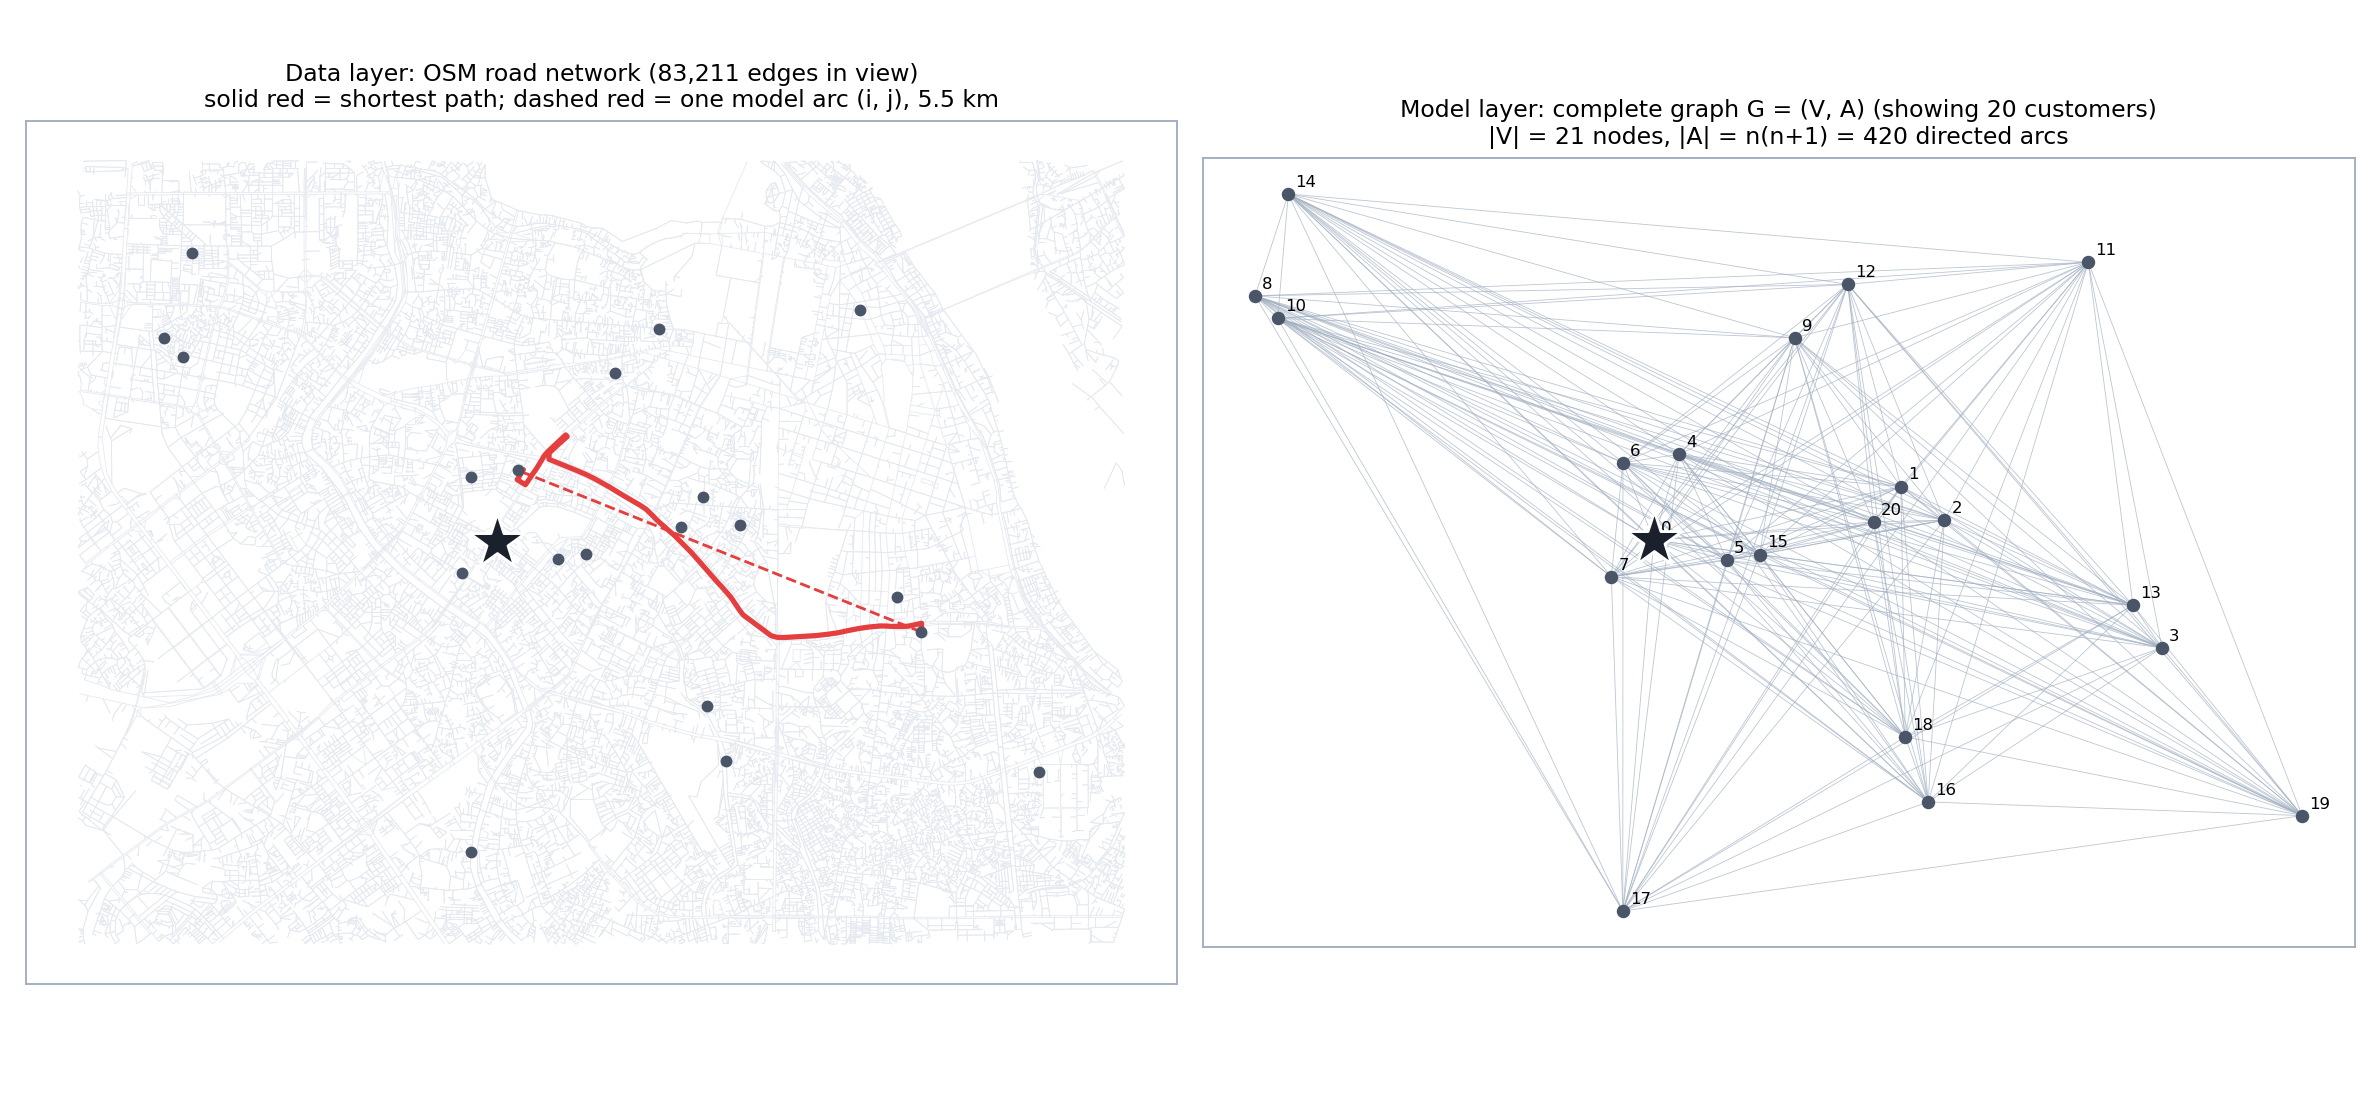
\includegraphics[width=0.75\linewidth]{figures/graph_layers.png}
    \caption{Left: the road network (data layer) and the fastest road path
    behind one model arc $(i,j)$. Right: the complete directed graph of the
    model (model layer) for the first 20 customers of INS\_XS.}
    \label{fig:graph}
\end{figure}

Five customer sets were generated with different seeds: MAIN (500
customers) and REP1--REP4 (200 each), from which nested instances are taken
(INS\_XS, INS\_S, INS\_M, INS\_L with 30, 80, 200 and 500 customers from
MAIN; REP$k$\_S and REP$k$\_M with 80 and 200 from REP$k$). To isolate the
effect of size, the experiments fix $|K|=2$, $B_{kt}=8$\,h, $m_i=2$ and the
base scenario, and use the first $n$ customers of INS\_XS ($n=10,20,30$) or
INS\_S ($n=50,80$). REP1\_S--REP4\_S (one day) and REP1\_S--REP2\_S (five
days) are added at $n=80$ to check that the conclusions do not depend on one
customer set.

\subsection{Computational Environment}
All experiments ran on a laptop with an Intel Core i7-1165G7 (2.80\,GHz, 4
cores), 8\,GB of memory and Windows~10, using Julia 1.13.2, JuMP 1.32.1 and
HiGHS.jl 1.26.0 (HiGHS 1.15.1) with default solver settings, under which the
MIP search is essentially serial. Two experiments ran in parallel as separate
single-threaded processes. Code, configurations and per-run results are in
the repository~\cite{projectrepo}.

\subsection{Experimental Protocol}
\textbf{Algorithm comparison.} \emph{Phase~1} solves a one-day problem
($H=1$, no day linking) and \emph{Phase~2} the five-day problem ($H=5$).
Each configuration is solved in 10 independent runs $r=1,\dots,10$ with seed
$2026+r$, shared by every method of that run; all values are averages over
the 10 runs. The HiGHS time limit is 30\,s in Phase~1 and
$150\,\text{s}=5\times30$\,s in Phase~2. The metaheuristics have the same
iteration budget: at most 300 iterations or generations, stopping after 50
consecutive iterations without improvement. In Phase~2, HiGHS is run twice
per run, cold and warm-started from the ALNS solution of the same seed. When
HiGHS proves optimality, the distance solve~\eqref{eq:lexi}--\eqref{eq:distance}
follows with the same time limit. Before any timing, every method is run once
on a five-customer instance so that Julia's compilation time is excluded.

\textbf{Timing.} The reported time is the wall-clock time of the solver call:
\texttt{optimize!} for the main HiGHS solve, and construction, search and
repair for the metaheuristics. Model building, the ALNS run that provides the
warm start and the distance solve are excluded; the distance solve time is
recorded separately~\cite{projectrepo}.

\textbf{Budget sensitivity.} To check that the 300/50 budget does not decide
the ranking, the Phase~2 runs on INS\_S with $n=80$ were repeated with five
times the budget (1{,}500 iterations, 250 without improvement).

\textbf{Policy comparison.} The routing method is fixed per experiment: the
best heuristic (ALNS) and the fastest one (Tabu) of Phase~2 at $n=80$, both
with the same 300/50 rule for the static plan and for every daily re-solve.
The instance is INS\_S ($n=80$, $K=2$, $H=5$, $m_i=2$) under three probability
scenarios with 20 payment scenarios each. The dataset stores a uniform number
$\xi^{(s)}_{it}\in[0,1]$ per customer and day; a visit succeeds if
$\xi^{(s)}_{it}<p_{it}$. All policies use the same numbers (common random
numbers), and the planners never see them. In the static policy, a planned
visit to a customer who has already paid is skipped and the freed time is
not reused.

\subsection{Evaluation Metrics}
\begin{itemize}
\item \textbf{Expected collection $Z$}, \textbf{simulated collection}
  (sum of $w_i$ over the successful visits in one payment scenario, used to
  compare policies), both in million VND, and \textbf{distance} in km.
\item \textbf{Optimality gap.} With $UB^\ast$ the tightest upper bound of the
  HiGHS calls in a run, the gap of every method in that run is
  \begin{equation}
  \mathrm{gap}=\frac{UB^\ast-Z}{Z}\times 100\%.
  \label{eq:gap}
  \end{equation}
  For the heuristics the gap is conservative, since $UB^\ast$ may be loose.
  In all 200 runs every method returned a feasible solution and HiGHS a
  finite bound.
\item \textbf{B\&B nodes} (\texttt{MOI.NodeCount}) of the main solve, and the
  number of runs out of 10 with status \texttt{OPTIMAL}.
\end{itemize}

\subsection{Algorithm Comparison}
Table~\ref{tab:algorithms} reports the main instances; $n=10$ and $n=20$
behave like $n=30$ (HiGHS optimal in 10/10 runs, every metaheuristic at the
optimum), and all per-run data are in the repository~\cite{projectrepo}.

\begin{table}[htbp]
\centering
\caption{Algorithm comparison over ten runs, mean $\pm$ standard deviation.
$Z$ in million VND, time in seconds, distance of the returned plan in km;
nodes are means. ``Warm'' is HiGHS started from ALNS.}
\label{tab:algorithms}
\scriptsize
\setlength{\tabcolsep}{3.5pt}
\begin{tabular}{@{}llrrrrrr@{}}
\toprule
Instance & Method & $Z$ & Time & Gap (\%) & Nodes & Opt. & km \\
\midrule
\multicolumn{8}{@{}l}{\textit{Phase 1: one day, 30\,s limit}} \\
INS\_XS, $n=30$ & HiGHS & 139.18\,$\pm$\,0.00 & 1.96\,$\pm$\,0.31 & 0.00\,$\pm$\,0.00 & 1.0 & 10/10 & 62.6\,$\pm$\,8.6 \\
 & GA & 139.18\,$\pm$\,0.00 & 3.00\,$\pm$\,0.69 & 0.00\,$\pm$\,0.00 & -- & -- & 53.3\,$\pm$\,3.0 \\
 & Tabu & 139.18\,$\pm$\,0.00 & 1.37\,$\pm$\,0.43 & 0.00\,$\pm$\,0.00 & -- & -- & 53.0\,$\pm$\,2.1 \\
 & ALNS & 139.18\,$\pm$\,0.00 & 1.32\,$\pm$\,0.52 & 0.00\,$\pm$\,0.00 & -- & -- & 51.2\,$\pm$\,0.8 \\
\midrule
INS\_S, $n=50$ & HiGHS & 68.39\,$\pm$\,41.62 & 30.80\,$\pm$\,0.20 & 273\,$\pm$\,171 & 3.8 & 0/10 & 33.6\,$\pm$\,27.6 \\
 & GA & 200.89\,$\pm$\,0.24 & 6.77\,$\pm$\,1.75 & 0.64\,$\pm$\,0.12 & -- & -- & 64.8\,$\pm$\,3.2 \\
 & Tabu & 200.83\,$\pm$\,0.28 & 2.44\,$\pm$\,1.00 & 0.67\,$\pm$\,0.15 & -- & -- & 66.2\,$\pm$\,4.2 \\
 & ALNS & 200.94\,$\pm$\,0.23 & 7.03\,$\pm$\,1.83 & 0.62\,$\pm$\,0.14 & -- & -- & 64.2\,$\pm$\,4.9 \\
\midrule
INS\_S, $n=80$ & HiGHS & 41.79\,$\pm$\,30.79 & 31.60\,$\pm$\,0.26 & 862\,$\pm$\,742 & 0.0 & 0/10 & 21.1\,$\pm$\,19.3 \\
 & GA & 274.32\,$\pm$\,0.96 & 7.97\,$\pm$\,2.66 & 2.40\,$\pm$\,0.37 & -- & -- & 65.5\,$\pm$\,3.1 \\
 & Tabu & 273.43\,$\pm$\,0.52 & 2.50\,$\pm$\,0.67 & 2.74\,$\pm$\,0.24 & -- & -- & 68.9\,$\pm$\,1.7 \\
 & ALNS & 274.81\,$\pm$\,0.61 & 14.32\,$\pm$\,4.54 & 2.22\,$\pm$\,0.22 & -- & -- & 63.6\,$\pm$\,4.5 \\
\midrule
\multicolumn{8}{@{}l}{\textit{Phase 2: five days, 150\,s limit}} \\
INS\_XS, $n=30$ & HiGHS & 246.80\,$\pm$\,0.00 & 16.85\,$\pm$\,17.59 & 0.00\,$\pm$\,0.00 & 56.5 & 10/10 & 144.0\,$\pm$\,10.5 \\
 & HiGHS warm & 246.80\,$\pm$\,0.00 & 1.28\,$\pm$\,0.18 & 0.00\,$\pm$\,0.00 & 0.0 & 10/10 & 103.2\,$\pm$\,2.3 \\
 & GA & 246.80\,$\pm$\,0.00 & 9.85\,$\pm$\,2.03 & 0.00\,$\pm$\,0.00 & -- & -- & 107.1\,$\pm$\,3.3 \\
 & Tabu & 246.80\,$\pm$\,0.00 & 2.72\,$\pm$\,1.31 & 0.00\,$\pm$\,0.00 & -- & -- & 111.5\,$\pm$\,3.2 \\
 & ALNS & 246.80\,$\pm$\,0.00 & 3.14\,$\pm$\,0.69 & 0.00\,$\pm$\,0.00 & -- & -- & 103.2\,$\pm$\,2.3 \\
\midrule
INS\_S, $n=50$ & HiGHS & 35.82\,$\pm$\,16.61 & 152.78\,$\pm$\,0.41 & 1{,}264\,$\pm$\,978 & 4.1 & 0/10 & 55.5\,$\pm$\,24.4 \\
 & HiGHS warm & 361.90\,$\pm$\,0.03 & 152.83\,$\pm$\,0.29 & 0.08\,$\pm$\,0.01 & 3.8 & 0/10 & 216.6\,$\pm$\,6.6 \\
 & GA & 361.59\,$\pm$\,0.14 & 14.31\,$\pm$\,3.77 & 0.16\,$\pm$\,0.04 & -- & -- & 266.6\,$\pm$\,9.4 \\
 & Tabu & 361.56\,$\pm$\,0.16 & 4.30\,$\pm$\,1.72 & 0.17\,$\pm$\,0.04 & -- & -- & 238.7\,$\pm$\,6.5 \\
 & ALNS & 361.90\,$\pm$\,0.03 & 8.03\,$\pm$\,2.97 & 0.08\,$\pm$\,0.01 & -- & -- & 216.6\,$\pm$\,6.6 \\
\midrule
INS\_S, $n=80$ & HiGHS & 6.99\,$\pm$\,6.70 & 156.64\,$\pm$\,0.27 & 16{,}594\,$\pm$\,15{,}341 & 0.0 & 0/10 & 4.2\,$\pm$\,2.7 \\
 & HiGHS warm & 549.04\,$\pm$\,0.22 & 156.53\,$\pm$\,0.28 & 0.38\,$\pm$\,0.04 & 0.0 & 0/10 & 329.1\,$\pm$\,12.4 \\
 & GA & 542.49\,$\pm$\,2.13 & 24.12\,$\pm$\,4.45 & 1.59\,$\pm$\,0.40 & -- & -- & 336.0\,$\pm$\,9.6 \\
 & Tabu & 545.20\,$\pm$\,0.58 & 6.27\,$\pm$\,1.05 & 1.09\,$\pm$\,0.11 & -- & -- & 352.1\,$\pm$\,6.7 \\
 & ALNS & 549.04\,$\pm$\,0.22 & 31.79\,$\pm$\,6.55 & 0.38\,$\pm$\,0.04 & -- & -- & 329.1\,$\pm$\,12.4 \\
\bottomrule
\end{tabular}
\end{table}

\begin{figure}[htbp]
    \centering
    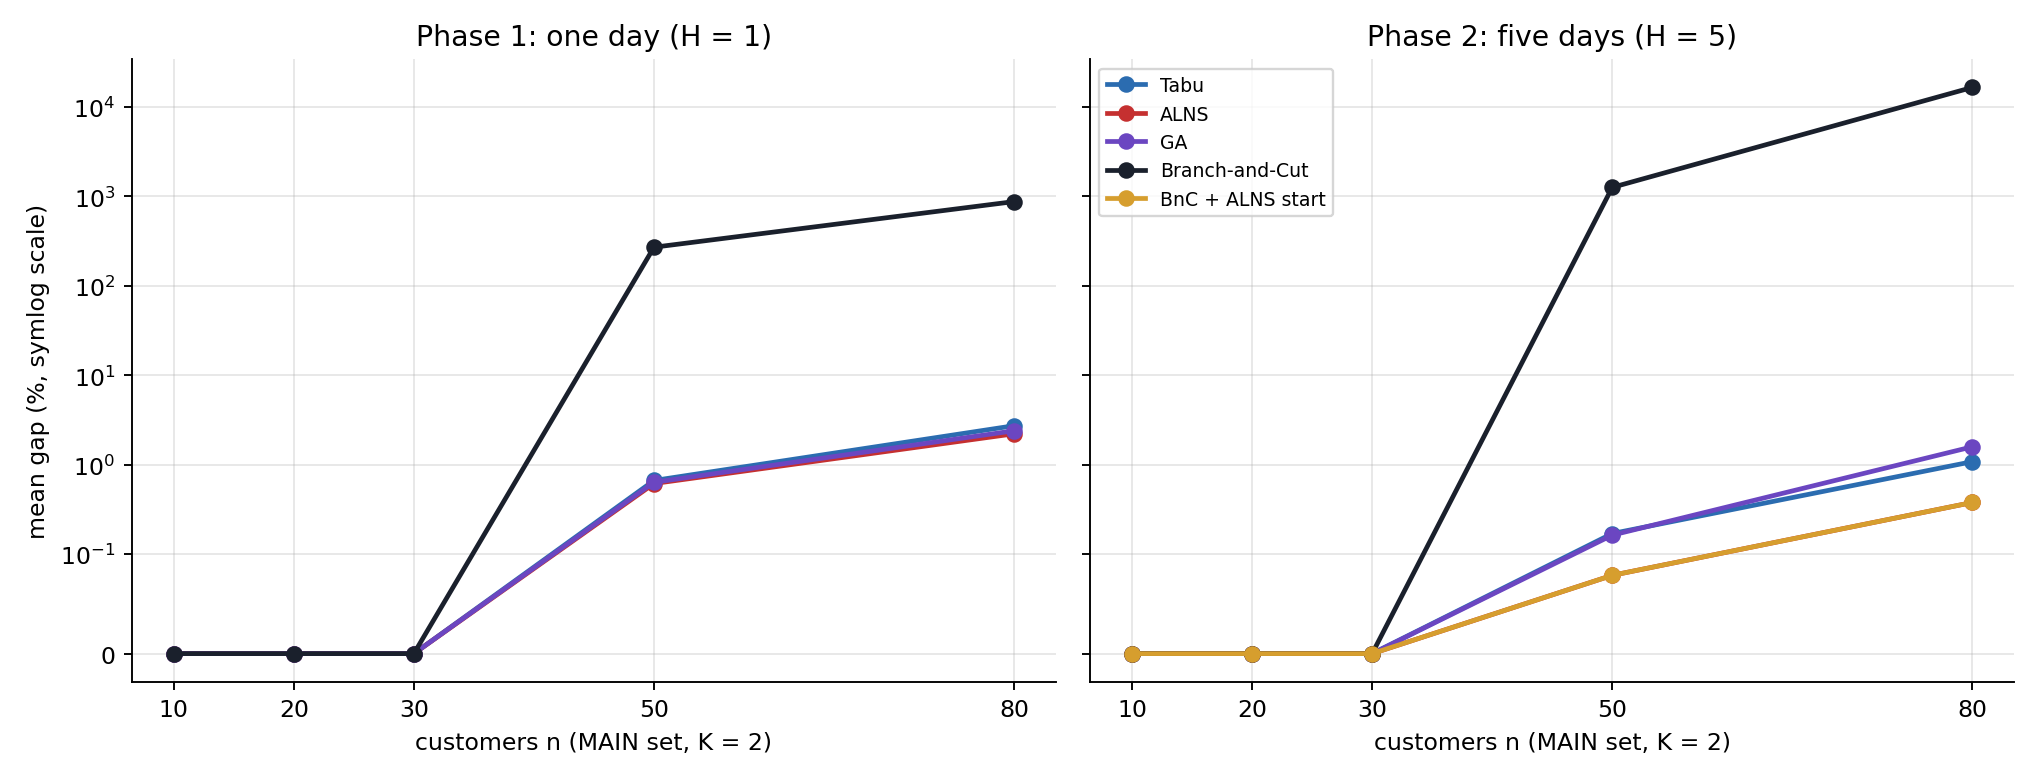
\includegraphics[width=0.85\linewidth]{figures/gap.png}
    \caption{Mean gap (symmetric log scale) against $n$ on the MAIN set.}
    \label{fig:gap-cpu}
\end{figure}

Figure~\ref{fig:gap-cpu} plots the gap against $n$.
Table~\ref{tab:replicates} repeats the $n=80$ comparison on independently
generated customer sets, and Table~\ref{tab:budget} gives the budget check.

\begin{table}[htbp]
\centering
\begin{minipage}[t]{0.575\linewidth}
\centering
\caption{Gap (\%) at $n=80$ on independent customer sets, mean $\pm$ standard deviation over ten runs (HiGHS: mean).}
\label{tab:replicates}
\scriptsize
\setlength{\tabcolsep}{1.5pt}
\begin{tabular}{@{}llrrrrr@{}}
\toprule
Ph. & Instance & HiGHS & Warm & GA & Tabu & ALNS \\
\midrule
1 & INS\_S & 862 & \NA & 2.40\,$\pm$\,0.37 & 2.74\,$\pm$\,0.24 & 2.22\,$\pm$\,0.22 \\
 & REP1\_S & 2{,}519 & \NA & 3.28\,$\pm$\,0.50 & 3.63\,$\pm$\,0.55 & 3.68\,$\pm$\,0.77 \\
 & REP2\_S & 1{,}112 & \NA & 3.31\,$\pm$\,0.32 & 3.71\,$\pm$\,0.41 & 3.70\,$\pm$\,0.47 \\
 & REP3\_S & 24{,}331 & \NA & 2.27\,$\pm$\,0.38 & 2.57\,$\pm$\,0.26 & 2.23\,$\pm$\,0.34 \\
 & REP4\_S & 5{,}911 & \NA & 2.70\,$\pm$\,0.10 & 2.73\,$\pm$\,0.37 & 2.70\,$\pm$\,0.12 \\
\midrule
2 & INS\_S & 16{,}594 & 0.38\,$\pm$\,0.04 & 1.59\,$\pm$\,0.40 & 1.09\,$\pm$\,0.11 & 0.38\,$\pm$\,0.04 \\
 & REP1\_S & 41{,}049 & 0.49\,$\pm$\,0.03 & 2.56\,$\pm$\,0.30 & 1.18\,$\pm$\,0.06 & 0.49\,$\pm$\,0.03 \\
 & REP2\_S & 14{,}769 & 0.45\,$\pm$\,0.03 & 2.21\,$\pm$\,0.45 & 1.01\,$\pm$\,0.06 & 0.45\,$\pm$\,0.03 \\
\bottomrule
\end{tabular}
\end{minipage}\hfill
\begin{minipage}[t]{0.415\linewidth}
\centering
\caption{Budget check, Phase~2, INS\_S, $n=80$: 300/50 against 1{,}500/250
iterations, mean $\pm$ standard deviation over ten runs.}
\label{tab:budget}
\scriptsize
\setlength{\tabcolsep}{1.5pt}
\begin{tabular}{@{}lrrrr@{}}
\toprule
 & \multicolumn{2}{c}{Gap (\%)} & \multicolumn{2}{c}{Time (s)} \\
\cmidrule(lr){2-3}\cmidrule(l){4-5}
Method & $1\times$ & $5\times$ & $1\times$ & $5\times$ \\
\midrule
GA & 1.59\,$\pm$\,0.40 & 0.87\,$\pm$\,0.20 & 24\,$\pm$\,4 & 181\,$\pm$\,39 \\
Tabu & 1.09\,$\pm$\,0.11 & 1.00\,$\pm$\,0.09 & 6\,$\pm$\,1 & 32\,$\pm$\,6 \\
ALNS & 0.38\,$\pm$\,0.04 & 0.33\,$\pm$\,0.03 & 32\,$\pm$\,7 & 238\,$\pm$\,67 \\
\bottomrule
\end{tabular}
\end{minipage}
\end{table}

\subsection{Static and Rolling-Horizon Comparison}
Table~\ref{tab:paired} gives the paired differences with 95\% confidence
intervals ($t$ distribution, 19 degrees of freedom). The expected value of
the static ALNS plan was 287.94, 549.49 and 783.45 million VND in the low,
base and high scenarios.

\begin{table}[htbp]
\centering
\caption{Policy comparison on INS\_S over 20 common payment scenarios.
Static: mean simulated collection (million VND). Rolling and myopic: mean
paired difference against static [95\% CI], number of scenarios out of 20
in which the policy collected more, and change in distance.}
\label{tab:paired}
\scriptsize
\setlength{\tabcolsep}{3pt}
\begin{tabular}{@{}llrrrrrr@{}}
\toprule
& & & \multicolumn{2}{c}{Rolling horizon} & \multicolumn{2}{c}{Myopic} & km \\
\cmidrule(lr){4-5}\cmidrule(lr){6-7}\cmidrule(l){8-8}
Scen. & Method & Static & Diff [95\% CI] & Better & Diff [95\% CI] & Better & R / M \\
\midrule
Low  & ALNS & 283.51 & $+4.9$ [$-3.0$, $12.8$] & 14 & $+5.7$ [$-0.6$, $11.9$] & 12 & $-5\%$ / $-12\%$ \\
     & Tabu & 274.71 & $+9.7$ [$-0.3$, $19.8$] & 10 & $+14.3$ [$-2.3$, $31.0$] & 11 & $-6\%$ / $-17\%$ \\
\midrule
Base & ALNS & 514.38 & $+2.3$ [$-4.3$, $8.8$] & 12 & $-6.4$ [$-21.1$, $8.3$] & 9 & $-9\%$ / $-17\%$ \\
     & Tabu & 490.49 & $+4.4$ [$-13.2$, $22.0$] & 11 & $\mathbf{+19.9}$ [$3.7$, $36.2$] & 16 & $-6\%$ / $-17\%$ \\
\midrule
High & ALNS & 735.90 & $+4.9$ [$-8.1$, $18.0$] & 11 & $-2.5$ [$-23.4$, $18.4$] & 9 & $-8\%$ / $-16\%$ \\
     & Tabu & 687.06 & $+12.5$ [$-13.4$, $38.4$] & 11 & $\mathbf{+47.7}$ [$20.9$, $74.4$] & 16 & $-7\%$ / $-19\%$ \\
\bottomrule
\end{tabular}
\end{table}

Per payment scenario, the optimization time was 43--57\,s for the static
ALNS plan, 58--89\,s for the five rolling-horizon re-solves and 28--54\,s for
the myopic ones; with Tabu the three figures were 5--9\,s, 13--19\,s and
5--9\,s.

\subsection{Discussion}
\textbf{Small instances.} Up to 30 customers, HiGHS proves optimality in
10/10 runs in both phases and the three metaheuristics find the same value
in every run. The one-day problem is solved at the root node, whereas the
five-day problem with 30 customers needs 56.5 nodes and 16.9\,s on average:
linking the days makes the problem much harder. Started from the ALNS
optimum, HiGHS needs only 1.3\,s.

\textbf{Distance.} The distance solve did not help HiGHS. At $n=20$ and
$n=30$ it always reached its time limit, and the cold HiGHS plan at $n=30$
is longer than the ALNS plan with the same $Z$ (62.6 against 51.2\,km in
Phase~1, 144.0 against 103.2\,km in Phase~2). For $n\ge50$ the cold HiGHS
plan is short only because it visits few customers.

\textbf{Behavior as size grows.} The model grows roughly as $|K|\,H\,n^2$,
from 2{,}012 variables ($n=30$, one day) to 67{,}610 ($n=80$, five days).
From $n=50$ on, HiGHS hits its time limit after at most 4 nodes on average,
and its incumbent is poor (gaps of 273\% to 16{,}594\% on INS\_S) and varies
a lot between runs. The bound is still informative: the heuristics lie
within 0.1--3.7\% of it, so the large gaps reflect the weak incumbent, not a
weak bound.

\textbf{Quality versus runtime.} At $n=80$ the metaheuristics reach gaps of
2.2--3.7\% in Phase~1 and 0.4--2.6\% in Phase~2 in 2 to 42\,s. In Phase~2,
ALNS gives the smallest gap on every instance with $n\ge50$ (0.08--0.49\%),
the smallest variation between runs and the shortest routes; Tabu is the
fastest (4--7\,s) at about 1\%; GA is slower than Tabu and has the largest
gap and variation at $n=80$. In Phase~1 the three methods are within about
0.5 percentage points and none is best everywhere. The REP sets give the
same picture. With five times the budget (Table~\ref{tab:budget}) GA gains
most (gap 1.59 to 0.87\%) and passes Tabu, while ALNS and Tabu gain less
than 0.1 point at 5--7.5 times the time. ALNS stays best, so the 300/50
budget does not change the main conclusion, but GA is the method most
limited by it.

For $n\ge50$, HiGHS started from ALNS returns exactly the ALNS solution:
within 150\,s it neither improves it nor closes the gap.

\textbf{Benefits and limits of re-optimization.} With ALNS, the rolling
horizon collects 0.4--1.7\% more than static in every scenario group, but
no confidence interval excludes 0. Its clear benefit is travel: 5--9\% less
distance, because planned repeat visits to customers who have already paid
are dropped. The myopic policy travels 12--17\% less, but with ALNS its collection
difference has a standard deviation of 13--45 million VND against 14--28 for
the rolling horizon, so it sometimes wins and sometimes loses by a large
margin. With Tabu, the static plan is weaker (3--7\% below ALNS) and
re-planning recovers much of the loss: the myopic policy collects
significantly more than static in the base and high scenarios
($+19.9$ and $+47.7$ million VND, 16/20 scenarios), reaching the level of
the ALNS policies. The one-day problems solved by the myopic policy are
small, where Tabu is close to the optimum, while its five-day static plan is
not. Re-planning thus matters most when the plan it replaces is weak. Two
factors limit the gain: each re-solve optimizes an expectation as if no
further re-planning will happen, and the variation between heuristic solves
is of the same order as the gain. Finally, the collection varies far more
between payment scenarios (standard deviation 150--220 million VND) than
between policies, so only paired differences on common random numbers can
separate them, and with 20 scenarios only differences of about 20 million
VND are detectable.

% ==================== 5. CONCLUSION ====================
\section{Conclusion}
\label{sec:conclusion}

This project modelled multi-officer, multi-day debt collection routing on
the road network of Hanoi as a MILP in which one precomputed visit schedule
is selected per customer, solved it with HiGHS, GA, Tabu search and ALNS,
and compared a static plan with rolling-horizon and myopic re-planning.

Up to 30 customers, HiGHS proves optimality within seconds and should be
preferred, since it gives a certificate. From 50 customers on, it stays at
the root node within 30--150\,s and its incumbent is unusable, but its bound
still measures the heuristics. At this size ALNS gives the best five-day
plans (gap 0.08--0.49\%, also the shortest routes) and Tabu slightly weaker
plans several times faster; five times more iterations do not change this.
Warm-starting HiGHS from ALNS did not improve the ALNS plan. On 80
customers, re-planning on top of ALNS did not change the simulated
collection significantly but cut travel by 5--9\% (rolling horizon) and
12--17\% (myopic); on top of the weaker Tabu plans, myopic re-planning raised
the collection significantly in two of the three scenarios.

Three lessons follow. First, a fast heuristic re-run every morning can
replace a strong one run once: Tabu with myopic re-planning collected within
2\% of the static ALNS plan in every scenario, with 8--12\% less travel and
5--10 times less computation. Second, the difficulty comes from linking the
days rather than from the number of customers, since with 30 customers the
one-day problem is solved at the root node while the five-day one needs 56
nodes; a decomposition by day is therefore the natural way to scale the
exact model. Third, HiGHS fails at finding good integer solutions, not at
bounding: its bound shows the heuristics to be at most 0.1--3.7\% from the
optimum,
so the practical combination is a heuristic for the plan and the MILP bound
as its quality certificate.

The customer accounts are synthetic, the payment probabilities are not
calibrated on real outcomes, travel speeds ignore congestion and payments
are full or nothing; the experiments stop at 80 customers, two officers and
20 payment scenarios. Natural next steps are the policy comparison with the
100 scenarios of the dataset on INS\_M and INS\_L, and stronger
subtour-elimination cuts or a decomposition by day to keep exact methods
usable beyond 30 customers.

% ==================== REFERENCES ====================

\begingroup
\small
\begin{thebibliography}{99}
\setlength{\itemsep}{0pt}

\bibitem{projectrepo}
N. T. Phuc and D. T. L. Huong,
\textit{Mathematic Modelling Project: Source Code and Data}.
Available at:
\url{https://github.com/PhucNT2511/Mathematic-modeling-project}.

\bibitem{osm}
OpenStreetMap contributors,
\textit{OpenStreetMap data for Vietnam} (Geofabrik extract
\texttt{vietnam-latest.osm.pbf}, data up to 18 October 2026),
Open Database License 1.0.
Available at: \url{https://download.geofabrik.de/asia/vietnam.html}.

\bibitem{nemotron}
NVIDIA,
\textit{Nemotron-Personas-Vietnam} [Dataset], CC BY 4.0,
revision \texttt{950724d}, accessed 20 October 2026.
Available at:
\url{https://huggingface.co/datasets/nvidia/Nemotron-Personas-Vietnam}.

\bibitem{uci2009}
I.-C. Yeh,
\textit{Default of Credit Card Clients} [Dataset],
UCI Machine Learning Repository, 2009.
DOI: \url{https://doi.org/10.24432/C55S3H}.

\bibitem{mtz1960}
C. E. Miller, A. W. Tucker, and R. A. Zemlin,
``Integer programming formulation of traveling salesman problems,''
\textit{Journal of the ACM}, vol.~7, no.~4, pp.~326--329, 1960.

\bibitem{ropke2006}
S. Ropke and D. Pisinger,
``An adaptive large neighborhood search heuristic for the pickup and
delivery problem with time windows,''
\textit{Transportation Science}, vol.~40, no.~4, pp.~455--472, 2006.

\bibitem{jump2023}
M. Lubin, O. Dowson, J. Dias Garcia, J. Huchette, B. Legat, and J. P. Vielma,
``JuMP 1.0: Recent improvements to a modeling language for mathematical
optimization,''
\textit{Mathematical Programming Computation}, vol.~15, pp.~581--589, 2023.

\bibitem{highs2018}
Q. Huangfu and J. A. J. Hall,
``Parallelizing the dual revised simplex method,''
\textit{Mathematical Programming Computation}, vol.~10, no.~1,
pp.~119--142, 2018.

\end{thebibliography}
\endgroup

\end{document}